%% LyX 2.0.5.1 created this file.  For more info, see http://www.lyx.org/.
%% Do not edit unless you really know what you are doing.
\documentclass{article}\usepackage{graphicx, color}
%% maxwidth is the original width if it is less than linewidth
%% otherwise use linewidth (to make sure the graphics do not exceed the margin)
\makeatletter
\def\maxwidth{ %
  \ifdim\Gin@nat@width>\linewidth
    \linewidth
  \else
    \Gin@nat@width
  \fi
}
\makeatother

\IfFileExists{upquote.sty}{\usepackage{upquote}}{}
\definecolor{fgcolor}{rgb}{0.2, 0.2, 0.2}
\newcommand{\hlnumber}[1]{\textcolor[rgb]{0,0,0}{#1}}%
\newcommand{\hlfunctioncall}[1]{\textcolor[rgb]{0.501960784313725,0,0.329411764705882}{\textbf{#1}}}%
\newcommand{\hlstring}[1]{\textcolor[rgb]{0.6,0.6,1}{#1}}%
\newcommand{\hlkeyword}[1]{\textcolor[rgb]{0,0,0}{\textbf{#1}}}%
\newcommand{\hlargument}[1]{\textcolor[rgb]{0.690196078431373,0.250980392156863,0.0196078431372549}{#1}}%
\newcommand{\hlcomment}[1]{\textcolor[rgb]{0.180392156862745,0.6,0.341176470588235}{#1}}%
\newcommand{\hlroxygencomment}[1]{\textcolor[rgb]{0.43921568627451,0.47843137254902,0.701960784313725}{#1}}%
\newcommand{\hlformalargs}[1]{\textcolor[rgb]{0.690196078431373,0.250980392156863,0.0196078431372549}{#1}}%
\newcommand{\hleqformalargs}[1]{\textcolor[rgb]{0.690196078431373,0.250980392156863,0.0196078431372549}{#1}}%
\newcommand{\hlassignement}[1]{\textcolor[rgb]{0,0,0}{\textbf{#1}}}%
\newcommand{\hlpackage}[1]{\textcolor[rgb]{0.588235294117647,0.709803921568627,0.145098039215686}{#1}}%
\newcommand{\hlslot}[1]{\textit{#1}}%
\newcommand{\hlsymbol}[1]{\textcolor[rgb]{0,0,0}{#1}}%
\newcommand{\hlprompt}[1]{\textcolor[rgb]{0.2,0.2,0.2}{#1}}%

\usepackage{framed}
\makeatletter
\newenvironment{kframe}{%
 \def\at@end@of@kframe{}%
 \ifinner\ifhmode%
  \def\at@end@of@kframe{\end{minipage}}%
  \begin{minipage}{\columnwidth}%
 \fi\fi%
 \def\FrameCommand##1{\hskip\@totalleftmargin \hskip-\fboxsep
 \colorbox{shadecolor}{##1}\hskip-\fboxsep
     % There is no \\@totalrightmargin, so:
     \hskip-\linewidth \hskip-\@totalleftmargin \hskip\columnwidth}%
 \MakeFramed {\advance\hsize-\width
   \@totalleftmargin\z@ \linewidth\hsize
   \@setminipage}}%
 {\par\unskip\endMakeFramed%
 \at@end@of@kframe}
\makeatother

\definecolor{shadecolor}{rgb}{.97, .97, .97}
\definecolor{messagecolor}{rgb}{0, 0, 0}
\definecolor{warningcolor}{rgb}{1, 0, 1}
\definecolor{errorcolor}{rgb}{1, 0, 0}
\newenvironment{knitrout}{}{} % an empty environment to be redefined in TeX

\usepackage{alltt}
\usepackage[sc]{mathpazo}
\usepackage{geometry}
\geometry{verbose,tmargin=2.5cm,bmargin=2.5cm,lmargin=2.5cm,rmargin=2.5cm}
\setcounter{secnumdepth}{2}
\setcounter{tocdepth}{2}
\usepackage{url}
\usepackage[unicode=true,pdfusetitle,
 bookmarks=true,bookmarksnumbered=true,bookmarksopen=true,bookmarksopenlevel=2,
 breaklinks=false,pdfborder={0 0 1},backref=false,colorlinks=false]
 {hyperref}
\hypersetup{
 pdfstartview={XYZ null null 1}}
\usepackage{breakurl}
\begin{document}





\title{Stat 2025- HW 4}
\author{Michael Discenza}

\maketitle

I first imported the data, added meaningful labels to the fields, and then took out the fertilizer field which we are not using.  I did some exploratory data analysis, plotting the distribtuions of some of the predictors and the response variable in order to get a sense of what models might be reasonable to fit to the data.
\begin{knitrout}
\definecolor{shadecolor}{rgb}{0.969, 0.969, 0.969}\color{fgcolor}\begin{kframe}
\begin{alltt}
tri <- \hlfunctioncall{read.table}(\hlstring{"http://www.stat.columbia.edu/~madigan/W2025/data/trinta2.dat"},na.string=\hlstring{"."})
\hlfunctioncall{colnames}(tri)[1] <- \hlstring{"weight"}
\hlfunctioncall{colnames}(tri)[2] <- \hlstring{"leaf.area"}
\hlfunctioncall{colnames}(tri)[3] <- \hlstring{"fertilizer"}
\hlfunctioncall{colnames}(tri)[4] <- \hlstring{"flower.count"}
\hlfunctioncall{colnames}(tri)[5] <- \hlstring{"daughter.count"}
\hlcomment{# we get rid of fertilizer}
tri$fertilizer <- NULL
tri <- \hlfunctioncall{na.omit}(tri)
\hlfunctioncall{library}(lattice)
\hlcomment{#\textbackslash{}pairs(tri)}
\hlfunctioncall{hist}(tri$daughter.count)
\hlfunctioncall{hist}(tri$weight)
\hlfunctioncall{hist}(tri$leaf)
\end{alltt}
\end{kframe}

{\centering 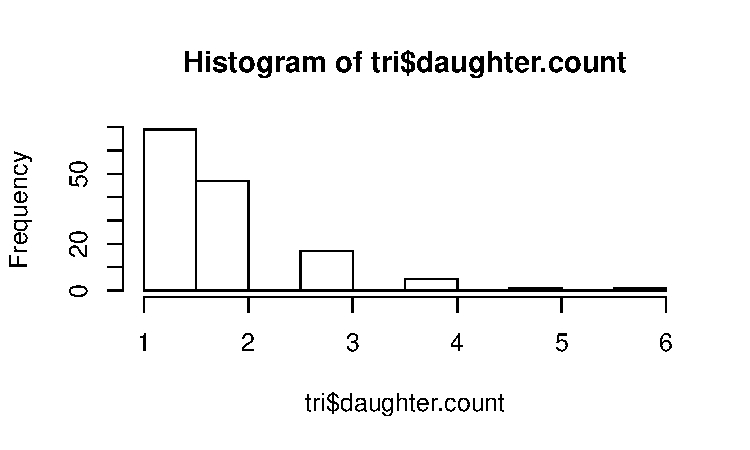
\includegraphics[width=\maxwidth]{figure/minimal-start1} 
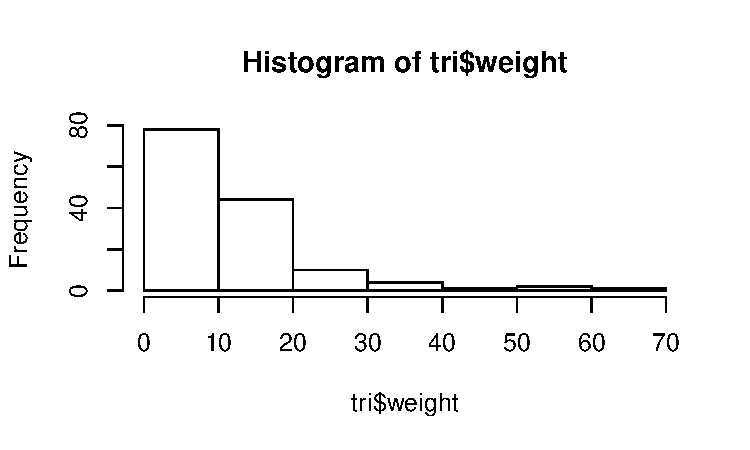
\includegraphics[width=\maxwidth]{figure/minimal-start2} 
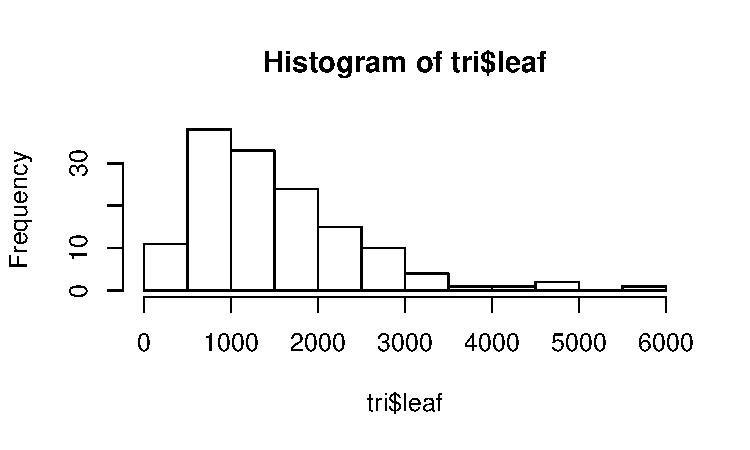
\includegraphics[width=\maxwidth]{figure/minimal-start3} 

}



\end{knitrout}

The response variable that we are interested in is the daughter count (shown in the historgram above).  That variable can only take the value zero and positive integer values so it makes sense to try to use a poisson regression model as the poisson distribution is a discrete distribution with the same properties.  Moreover, the fact that the mean is less than 10 suggests that poisson regression could potentially be ideal.

Before we choose which features to include in our model, it is important to see if any tansformations of the data would help.
\begin{knitrout}
\definecolor{shadecolor}{rgb}{0.969, 0.969, 0.969}\color{fgcolor}\begin{kframe}
\begin{alltt}

\hlfunctioncall{summary}(m1a <- \hlfunctioncall{glm}(daughter.count ~ weight, family = \hlstring{"poisson"}, data = tri))
\hlfunctioncall{plot}(m1a, which = 2)
\hlfunctioncall{plot}(m1a$residuals ~ tri$weight)
(m1a$null.deviance - m1a$deviance)/m1a$null.deviance

\hlfunctioncall{summary}(m1b <- \hlfunctioncall{glm}(daughter.count ~ \hlfunctioncall{log}(weight), family = \hlstring{"poisson"}, data = tri))
\hlfunctioncall{plot}(m1b, which = 2)
\hlfunctioncall{plot}(m1b$residuals ~ tri$weight)
(m1b$null.deviance - m1b$deviance)/m1b$null.deviance

\hlfunctioncall{summary}(m2a <- \hlfunctioncall{glm}(daughter.count ~ leaf.area, family = \hlstring{"poisson"}, data = tri))
\hlfunctioncall{plot}(m2a, which = 2)
(m2a$null.deviance - m2a$deviance)/m2a$null.deviance
\hlfunctioncall{summary}(m2b <- \hlfunctioncall{glm}(daughter.count ~ \hlfunctioncall{log}(leaf.area), family = \hlstring{"poisson"}, data = tri))
\hlfunctioncall{plot}(m2b, which = 2)
\hlcomment{# plot(m2)}
(m2b$null.deviance - m2b$deviance)/m2b$null.deviance
\hlcomment{# it's interesting that this is actually lower than the the data for the untransformed}
\hlcomment{# data, even though the residuals seem more normal}

\hlfunctioncall{summary}(m3 <- \hlfunctioncall{glm}(daughter.count ~ flower.count, family = \hlstring{"poisson"}, data = tri))
\hlcomment{# plot(m3)}
\hlfunctioncall{plot}(m3, which = 2)
\hlfunctioncall{plot}(m2$residuals ~ tri$flower.count)
\end{alltt}


{\ttfamily\noindent\bfseries\color{errorcolor}{\#\# Error: object 'm2' not found}}\begin{alltt}
(m3$null.deviance - m3$deviance)/m3$null.deviance
\hlfunctioncall{plot}(tri$daughter.count ~ tri$leaf.area)
\end{alltt}
\end{kframe}
\end{knitrout}

I tried fitting the single predictor models with log and exponential transofrmations of the data (Prof. Madigan said it might be a good idea in class or that it was possible to do this, but I was not able to figure out why from reading the text book and sources online. I think that part of it could be that though we are trying to find the MLE for the parameter of a poisson distribution, but the error function perahps is still assumed to be chracterized by a Gaussian distribution[??].  This means that we should ideally still see residuals distributed normally.) In any case though, the transofrmations seemed ineffective.  For example, in fitting a single predictor model using the log of leaf area, the QQ-norm plot looked much better, indicating that the residuals were more normally distributed that the model using fit to the untransformed data, but alarmingly, the the the explained deviance dropped by an order of magnitude for the model with the transofrmed leaf area vector.  

I conducted the procedure below for a number of different versions of log transformed data. For the log(weight), none of the combinations of predictors reached the levels of cross-validation prediction error that were achieved using untransofmed data.  When I used log(leaf.area) instead of leaf.area, I achieved a slightly better cross-validation prediction error, 0.740 vs. 0.752 for the untranformed data.  Interestingly though, the AIC and BIC figures for the log transformed model for daughter.count \string~ weight+log(leaf.area) vs. daughter.count \string~ weight+leaf.area are actually higher for the log transformed data (though not by much- for AIC, 390.37 vs. 389.87 and for BIC,  399.19 vs. 398.69), showing that those model selection criteria prefer the non-transofmed data.

I ended up choosing the model that used the log transformed vector of leaf.areas because the prediction error improvment is greater than the decreased AIC and BIC and because prediction error could be interepted as a more important metric depending on the use of the model.

I fit models for each combination of preditors and then compared the AIC, BIC, cross-validation prediction error, and explained deviance figure for each of the mdoels.  This approach worked for this small data set, but would not work if we had more predictors.

\begin{knitrout}
\definecolor{shadecolor}{rgb}{0.969, 0.969, 0.969}\color{fgcolor}\begin{kframe}
\begin{alltt}
tri$leaf.area <- \hlfunctioncall{log}(tri$leaf.area)
\hlfunctioncall{colnames}(tri)[2] <- \hlstring{"log.leaf.area"}
all_possible_models <- \hlfunctioncall{function}(x.column.names, y.col.name) \{
    Cols <- x.column.names
    n <- \hlfunctioncall{length}(Cols)
    id <- \hlfunctioncall{unlist}(\hlfunctioncall{lapply}(1:n, \hlfunctioncall{function}(i) \hlfunctioncall{combn}(1:n, i, simplify = F)), recursive = F)
    Formulas <- \hlfunctioncall{sapply}(id, \hlfunctioncall{function}(i) \hlfunctioncall{paste}(y.col.name, \hlstring{"~"}, \hlfunctioncall{paste}(Cols[i], collapse = \hlstring{"+"})))
    Formulas <- \hlfunctioncall{c}(Formulas, \hlfunctioncall{paste}(y.col.name, \hlstring{"~1"}))
\}

\hlfunctioncall{library}(boot)
\end{alltt}


{\ttfamily\noindent\itshape\color{messagecolor}{\#\# \\\#\# Attaching package: 'boot'}}

{\ttfamily\noindent\itshape\color{messagecolor}{\#\# The following object(s) are masked from 'package:lattice':\\\#\# \\\#\#\ \ \ \  melanoma}}\begin{alltt}
fit_models <- \hlfunctioncall{function}(model) \{
\hlcomment{    #make the default value for this function 5}
    fitmodel <- \hlfunctioncall{glm}(model, family = \hlstring{"poisson"}, data = tri)
    CVPE <- \hlfunctioncall{cv.glm}(tri, fitmodel, K = 5)$delta[2]
    AIC <- fitmodel$aic
    BIC <- \hlfunctioncall{BIC}(fitmodel)
    ED <- (fitmodel$null.deviance - fitmodel$deviance)/fitmodel$null.deviance
    result <- \hlfunctioncall{c}(ED, AIC, BIC, CVPE)
    \hlfunctioncall{return}(result)
\}

FORMULAS <- \hlfunctioncall{all_possible_models}(x.column.names = \hlfunctioncall{colnames}(tri[1:3]), y.col.name = \hlfunctioncall{colnames}(tri[4]))

model.summary <- \hlfunctioncall{as.data.frame}(\hlfunctioncall{lapply}(X = FORMULAS, fit_models))
\hlfunctioncall{names}(model.summary) <- NULL
model.summary <- \hlfunctioncall{cbind}(FORMULAS, \hlfunctioncall{t}(model.summary))
\hlfunctioncall{colnames}(model.summary)[2] <- \hlstring{"Explained Deviance"}
\hlfunctioncall{colnames}(model.summary)[3] <- \hlstring{"AIC"}
\hlfunctioncall{colnames}(model.summary)[4] <- \hlstring{"BIC"}
\hlfunctioncall{colnames}(model.summary)[5] <- \hlstring{"CVPE"}
model.summary <- \hlfunctioncall{as.data.frame}(model.summary)
model.summary
\end{alltt}
\begin{verbatim}
##                                             FORMULAS    Explained Deviance
## 1                            daughter.count ~ weight    0.0303595405361379
## 2                     daughter.count ~ log.leaf.area    0.0909193926729046
## 3                      daughter.count ~ flower.count    0.0787215216579329
## 4              daughter.count ~ weight+log.leaf.area     0.196208780760651
## 5               daughter.count ~ weight+flower.count     0.121790520108012
## 6        daughter.count ~ log.leaf.area+flower.count     0.113482943002382
## 7 daughter.count ~ weight+log.leaf.area+flower.count     0.209899507407305
## 8                                  daughter.count ~1 -2.32182056234451e-16
##                AIC              BIC              CVPE
## 1 398.519769502233 404.403054347452 0.865470804039708
## 2 394.813164115723 400.696448960941 0.822463940881569
## 3 395.559742794712 401.443027639931 0.825504689589662
## 4  390.36885820581 399.193785473637 0.755383809598388
## 5 394.923676555875 403.748603823703 0.796415873435106
## 6 395.432147249942  404.25707451777 0.829114131875539
## 7 391.530908320808 403.297478011245 0.760424939159392
## 8 398.377945051095 401.319587473705 0.889285714300621
\end{verbatim}
\end{kframe}
\end{knitrout}


Based on the results, it seems like the best model would be daughter.count ~ weight+log(leaf.area).  Though it does not hav highest explianed deviance, it has the the lowest AIC, BIC, and cross-validation predication error indicating that it is the most use useful.

We can also use a hypothesis testing approach to looking at what variables should be included in the model:

\begin{knitrout}
\definecolor{shadecolor}{rgb}{0.969, 0.969, 0.969}\color{fgcolor}\begin{kframe}
\begin{alltt}
m4 <- \hlfunctioncall{glm}(daughter.count ~ weight + log.leaf.area + flower.count, family = \hlstring{"poisson"}, data = tri)
\hlfunctioncall{drop1}(m4, test = \hlstring{"Chisq"})
\end{alltt}
\begin{verbatim}
## Single term deletions
## 
## Model:
## daughter.count ~ weight + log.leaf.area + flower.count
##               Df Deviance AIC  LRT Pr(>Chi)  
## <none>               48.4 392                
## weight         1     54.3 395 5.90    0.015 *
## log.leaf.area  1     53.8 395 5.39    0.020 *
## flower.count   1     49.2 390 0.84    0.360  
## ---
## Signif. codes:  0 '***' 0.001 '**' 0.01 '*' 0.05 '.' 0.1 ' ' 1
\end{verbatim}
\end{kframe}
\end{knitrout}

Passing in the full model with tall of the predictors, we see that, like the results from the previous approach to model selection, testing each of the variables' signifiance shows that we should include both weight and leaf.area, but not flower.count.

Our final model is:
\begin{knitrout}
\definecolor{shadecolor}{rgb}{0.969, 0.969, 0.969}\color{fgcolor}\begin{kframe}
\begin{alltt}
\hlfunctioncall{summary}(final.model <- \hlfunctioncall{glm}(daughter.count ~ weight + log.leaf.area, family = \hlstring{"poisson"}, data = tri))
\end{alltt}
\begin{verbatim}
## 
## Call:
## glm(formula = daughter.count ~ weight + log.leaf.area, family = "poisson", 
##     data = tri)
## 
## Deviance Residuals: 
##    Min      1Q  Median      3Q     Max  
## -1.170  -0.478  -0.149   0.344   1.835  
## 
## Coefficients:
##               Estimate Std. Error z value Pr(>|z|)   
## (Intercept)    -1.8398     0.8054   -2.28   0.0224 * 
## weight         -0.0179     0.0075   -2.39   0.0169 * 
## log.leaf.area   0.3621     0.1148    3.15   0.0016 **
## ---
## Signif. codes:  0 '***' 0.001 '**' 0.01 '*' 0.05 '.' 0.1 ' ' 1 
## 
## (Dispersion parameter for poisson family taken to be 1)
## 
##     Null deviance: 61.206  on 139  degrees of freedom
## Residual deviance: 49.197  on 137  degrees of freedom
## AIC: 390.4
## 
## Number of Fisher Scoring iterations: 4
\end{verbatim}
\end{kframe}
\end{knitrout}


The coefficients that we fit represent the estimated log change in the expected counts for a unit change in the predictor when all other predictors are held constant.

\begin{knitrout}
\definecolor{shadecolor}{rgb}{0.969, 0.969, 0.969}\color{fgcolor}\begin{kframe}
\begin{alltt}
\hlfunctioncall{exp}(final.model$coefficients[2])
\end{alltt}
\begin{verbatim}
## weight 
## 0.9823
\end{verbatim}
\begin{alltt}
\hlfunctioncall{exp}(final.model$coefficients[3])
\end{alltt}
\begin{verbatim}
## log.leaf.area 
##         1.436
\end{verbatim}
\begin{alltt}

\end{alltt}
\end{kframe}
\end{knitrout}


So for the coefficient for weight, in increase of 1 miligram, the count of daughters is expected to decrease by .982.  For the coefficient for leaf area, the interpetation is slightly different because we took the log of the predictor before fitting the model: a unit increase in the log area of the leaf results in increase of the expected count by 1.436301.



keep the increase in terms of log units

\end{document}
